% -*- latex -*-
%%%%%%%%%%%%%%%%%%%%%%%%%%%%%%%%%%%%%%%%%%%%%%%%%%%%%%%%%%%%%%%%
%%%%%%%%%%%%%%%%%%%%%%%%%%%%%%%%%%%%%%%%%%%%%%%%%%%%%%%%%%%%%%%%
%%%%
%%%% This text file is part of the source of 
%%%% `Parallel Computing'
%%%% by Victor Eijkhout, copyright 2012-6
%%%%
%%%% mpi-data.tex : discussion of MPI datatypes
%%%%
%%%%%%%%%%%%%%%%%%%%%%%%%%%%%%%%%%%%%%%%%%%%%%%%%%%%%%%%%%%%%%%%
%%%%%%%%%%%%%%%%%%%%%%%%%%%%%%%%%%%%%%%%%%%%%%%%%%%%%%%%%%%%%%%%

\index{datatype|(}

In the examples you have seen so far, every time data was sent,
it was as a contiguous buffer with elements of a single type.
In practice you may want to send heterogeneous data, or
non-contiguous data.
Figure~\ref{fig:blasmatrix} indicates one source of irregular
data:
%
\begin{figure}[ht]
  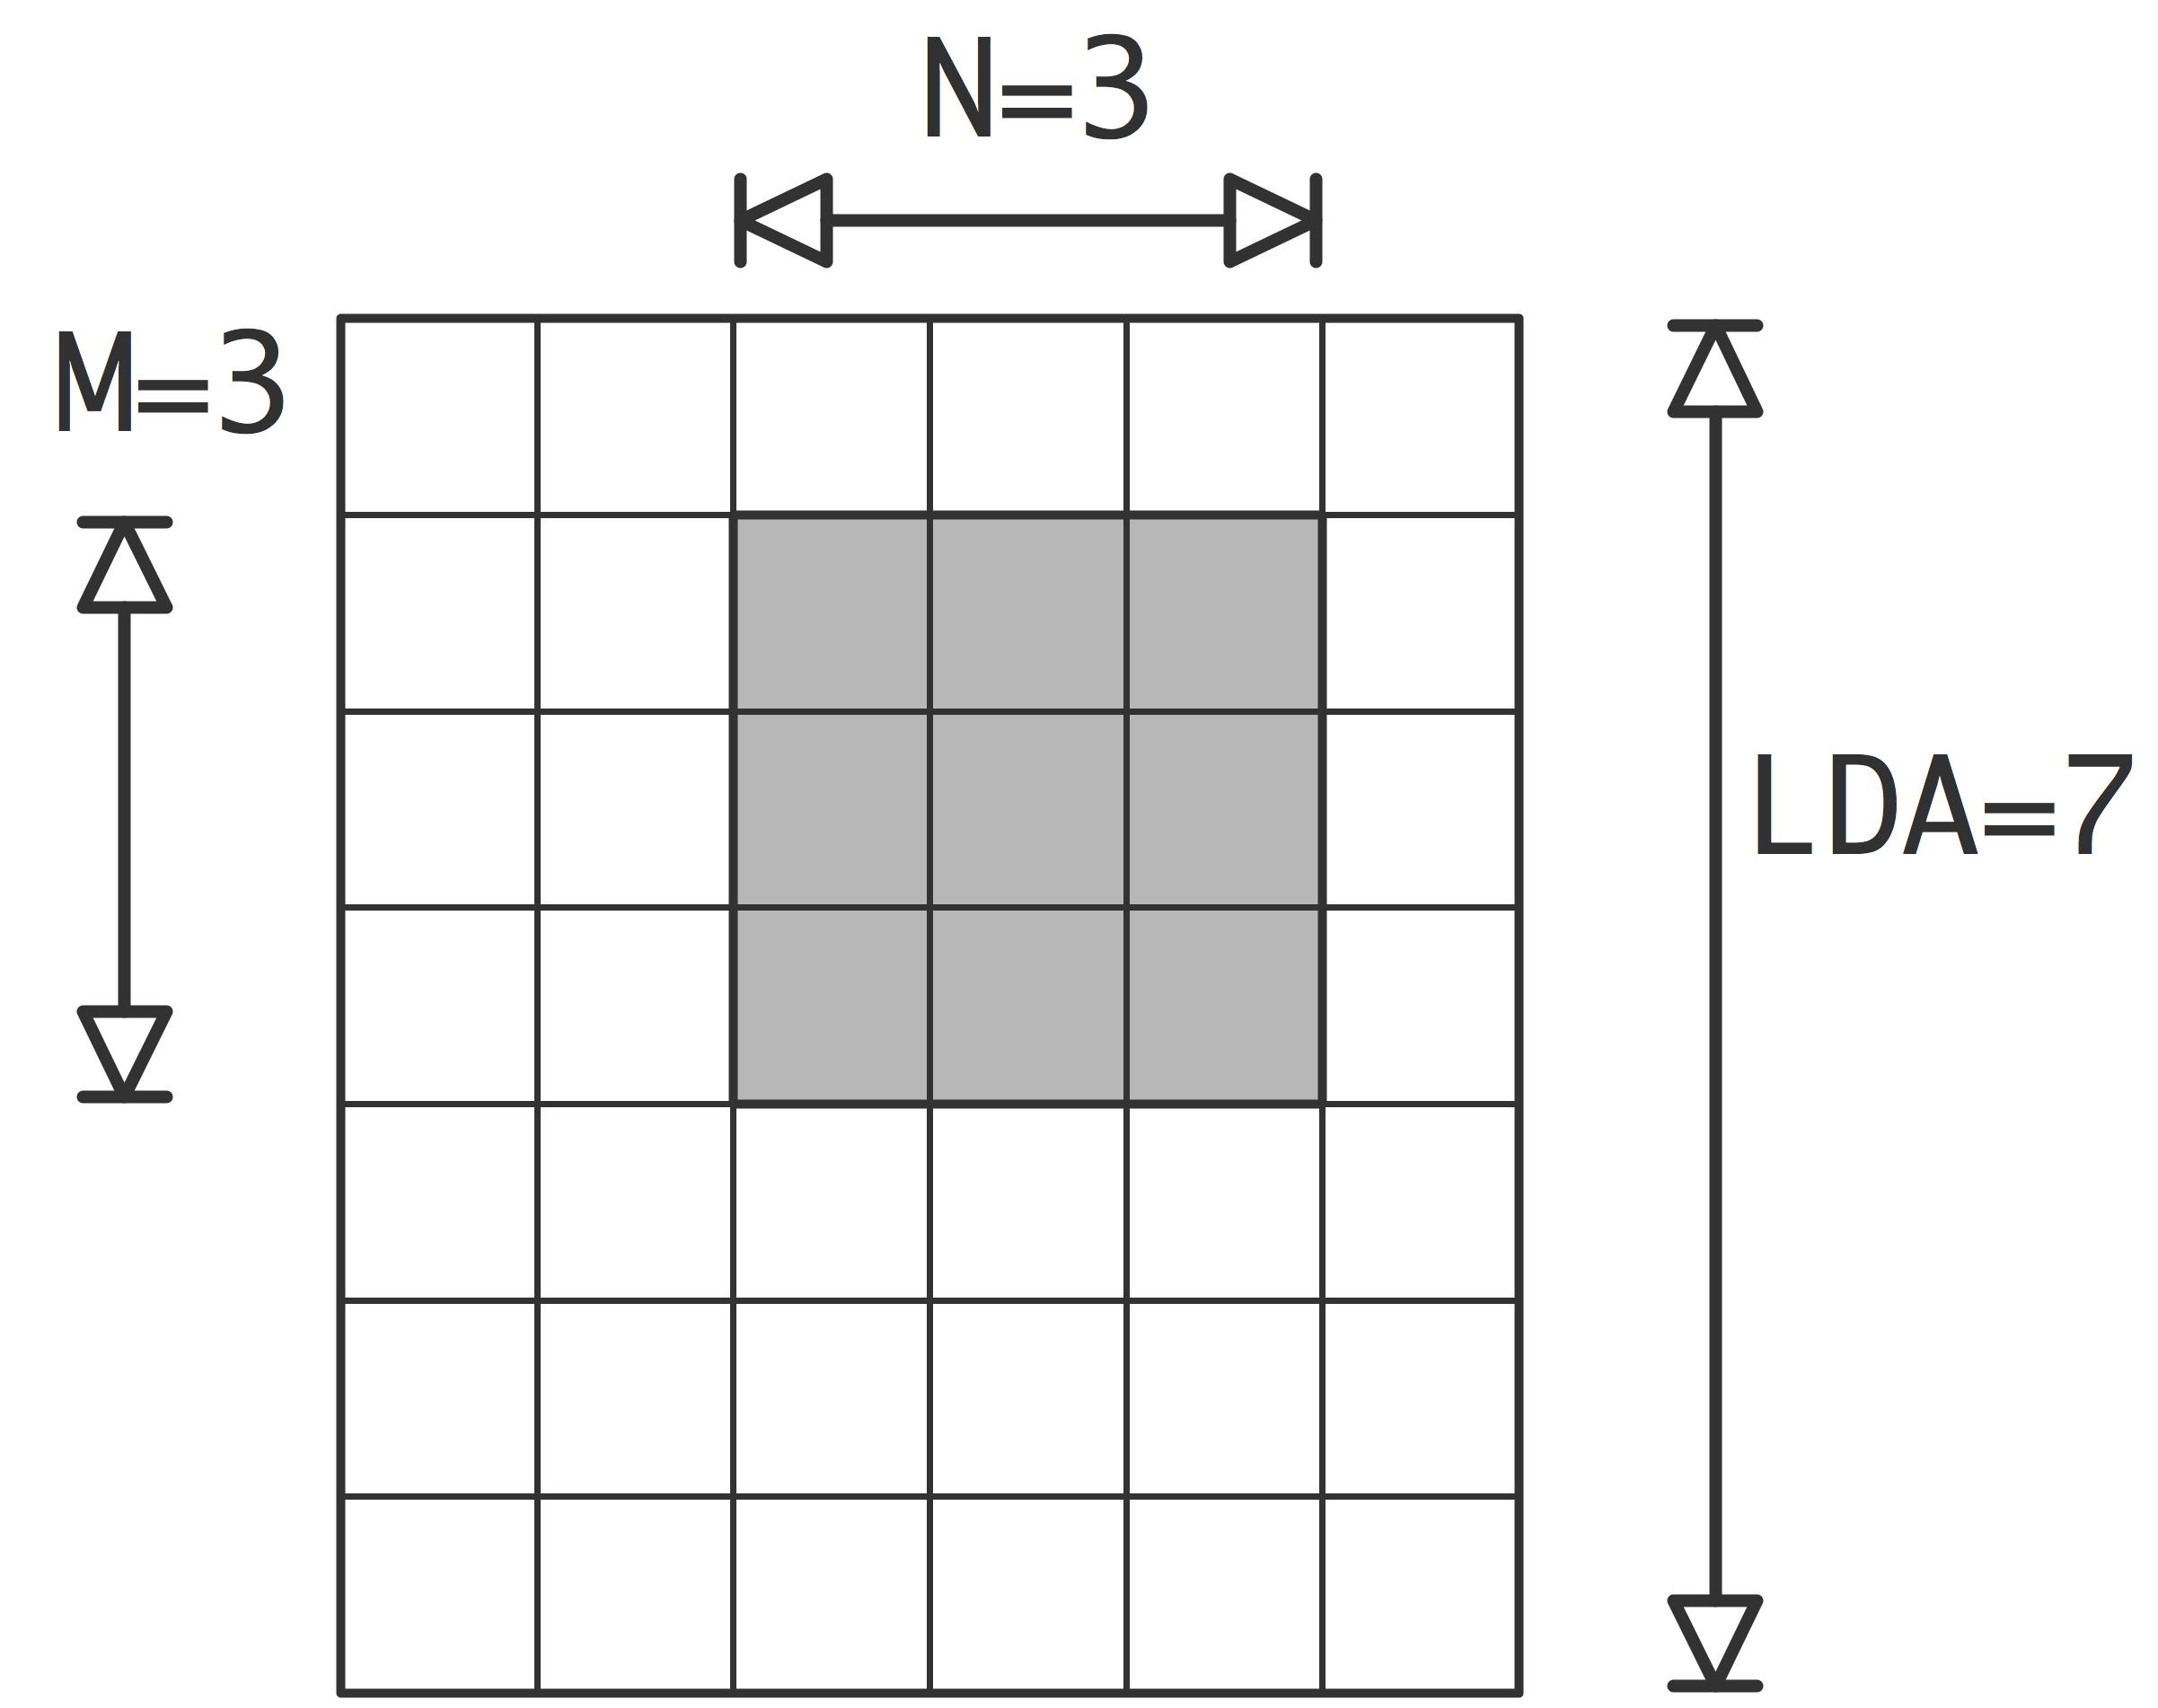
\includegraphics[scale=.1]{blasmatrix}
  \caption{Memory layout of a row and column of a matrix in column-major storage}
  \label{fig:blasmatrix}
\end{figure}
%
with a matrix on \indexterm{column-major storage}, a column is
stored in contiguous memory. However, a row of such a matrix
is not contiguous; its elements being separated by a \indexterm{stride}
equal to the column length.

\begin{exercise}
  \label{ex:submatrix}
  How would you describe the memory layout of a submatrix,
  if the whole matrix has size $M\times N$ and the submatrix $m\times n$?
\end{exercise}

The datatypes you have dealt with so far are known as
\indextermsub{elementary}{datatypes}; irregular objects
are known as \indextermsub{derived}{datatypes}.

\Level 0 {Elementary data types}
\commandref{elementary}
\index{datatype!elementary|(}

MPI has a number of elementary data types, corresponding to the 
simple data types of programming languages.
The names are made to resemble the types of C and~Fortran, 
for instance \n{MPI_FLOAT} and \n{MPI_DOUBLE} versus
\n{MPI_REAL} and \n{MPI_DOUBLE_PRECISION}.

MPI calls accept arrays of elements:
\begin{verbatim}
double x[20];
MPI_Send( x,20,MPI_DOUBLE, ..... )
\end{verbatim}
so for a single element you need to take its address:
\begin{verbatim}
double x;
MPI_Send( &x,1,MPI_DOUBLE, ..... )
\end{verbatim}

\index{datatype!elementary|)}

\Level 0 {Derived datatypes}
\commandref{derived-types}
\index{datatype!derived|(}

MPI allows you to create your own data types, somewhat (but not completely\ldots)
analogous to defining
structures in a programming language. MPI data types are mostly of use
if you want to send multiple items in one message.

There are two problems with using only elementary datatypes
as you have seen so far.
\begin{itemize}
\item MPI communication routines can only send multiples of a
  single data type: it is not possible to send items of different
  types, even if they are contiguous in memory. It would be possible
  to use the \n{MPI_BYTE} data type, but this is not advisable.
\item It is also ordinarily not possible to send items of one type if they are
  not contiguous in memory. You could of course send a contiguous memory area
  that contains the items you want to send, but that is wasteful of
  bandwidth.
\end{itemize}
With MPI data types you can solve these problems in several ways.
\begin{itemize}
\item You can create a new \indextermbus{contiguous}{data type}
  consisting of an array of elements of another data type. There is no
  essential difference between sending one element of such a type
  and multiple elements of the
  component type.
\item You can create a \indextermbus{vector}{data type} consisting of
  regularly spaced blocks of elements of a component type. This is a first
  solution to the problem of sending non-contiguous data.
\item For not regularly spaced data, there is the
  \indextermbus{indexed}{data type}, where you specify an array of
  index locations for blocks of elements of a component type.
  The blocks can each be of a different size.
\item The \indextermbus{struct}{data type} can accomodate multiple
  data types.
\end{itemize}
And you can combine these mechanisms to get irregularly spaced
heterogeneous data, et cetera.

\Level 1 {Datatype signatures}
\label{sec:signature}
\index{datatype!signature|(}

With the primitive types you have seen so far, it pretty much went
without saying that if the sender sends an array of doubles, the
receiver had to declare the datatype also as doubles. With derived
types that is no longer the case: the sender and receiver can declare
a different datatype for the send and receive buffer, as long as these
have the same \indextermbus{datatype}{signature}.

The signature of a datatype is the internal representation of that
datatype. For instance, if the sender declares a datatype consisting
of two doubles, and it sends four elements of that type, the receiver
can receive it as two elements of a type consisting of four doubles.

You can also look at the signature as the form `under the hood' in which MPI
sends the data.

\index{datatype!signature|)}

\Level 1 {Basic calls}
\commandref{data-commit}

New MPI data types are created by
\begin{itemize}
\item \indexmpishow{MPI_Type_contiguous}
\item \indexmpishow{MPI_Type_create_subarray}
\item \indexmpishow{MPI_Type_vector}
\item \indexmpishow{MPI_Type_struct}
\item \indexmpishow{MPI_Type_indexed}
\item \indexmpishow{MPI_Type_hindexed}
\end{itemize}
It is necessary to call \indexmpishow{MPI_Type_commit} which makes MPI
do the indexing calculations for the data type.  When you no longer
need the data type, you call \indexmpishow{MPI_Type_free}.

\Level 1 {Contiguous type}
\commandref{data:contiguous}

The simplest derived type is the `contiguous' type,
constructed with \indexmpishow{MPI_Type_contiguous}
A~contigous type describes an array of items
of an elementary or earlier defined type. There is no difference between sending
one item of a contiguous type and multiple items of the constituent type.
\begin{figure}[ht]
  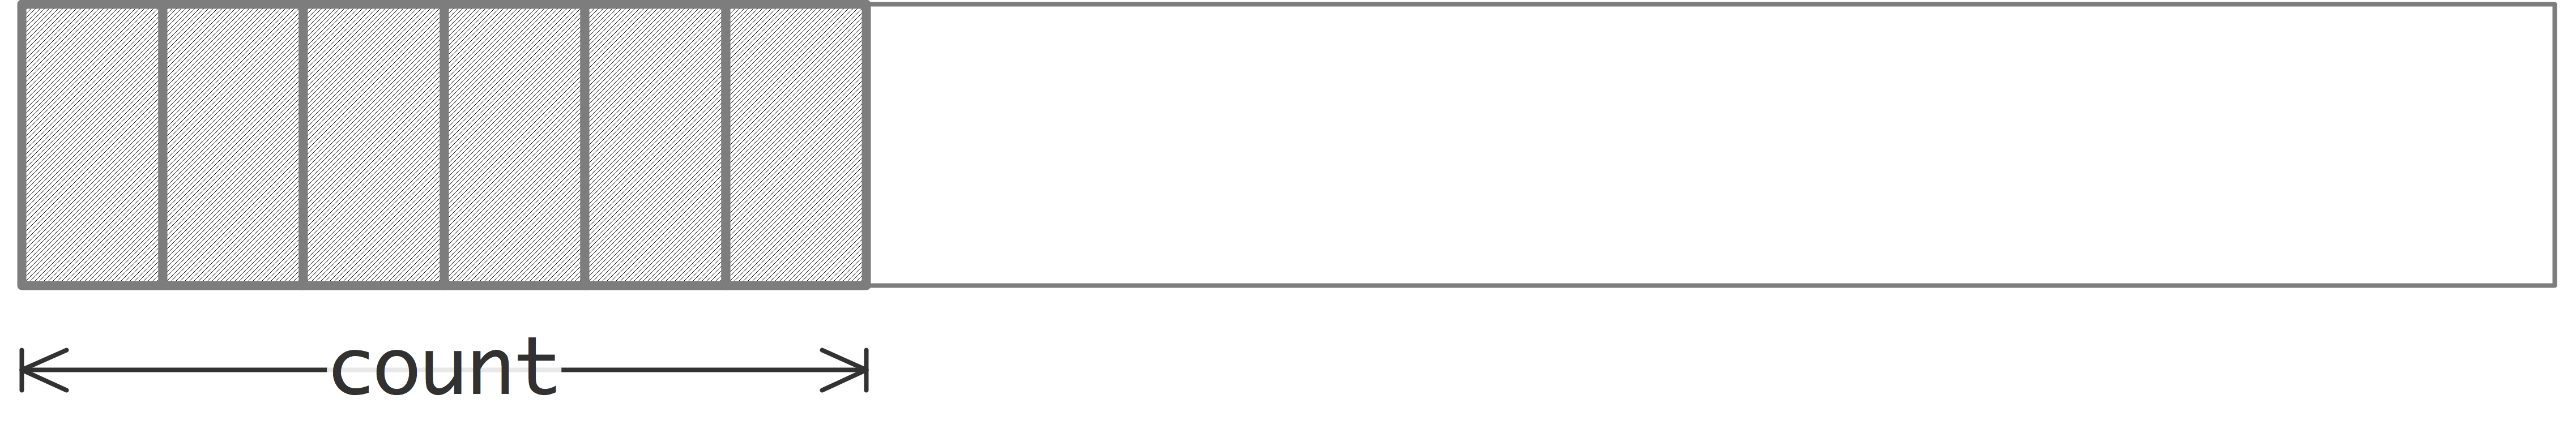
\includegraphics[scale=.08]{data-contiguous}
  \caption{A contiguous datatype is built up out of elements of a constituent type}
  \label{fig:data-contiguous}
\end{figure}
This is illustrated in figure~\ref{fig:data-contiguous}.

\Level 1 {Vector type}
\commandref{data:vector}

The simplest non-contiguous datatype is the `vector' type, constructed with
\indexmpishow{MPI_Type_vector}. A~vector type describes a series of blocks, all 
of equal size, spaced with a constant stride.
\begin{figure}[ht]
  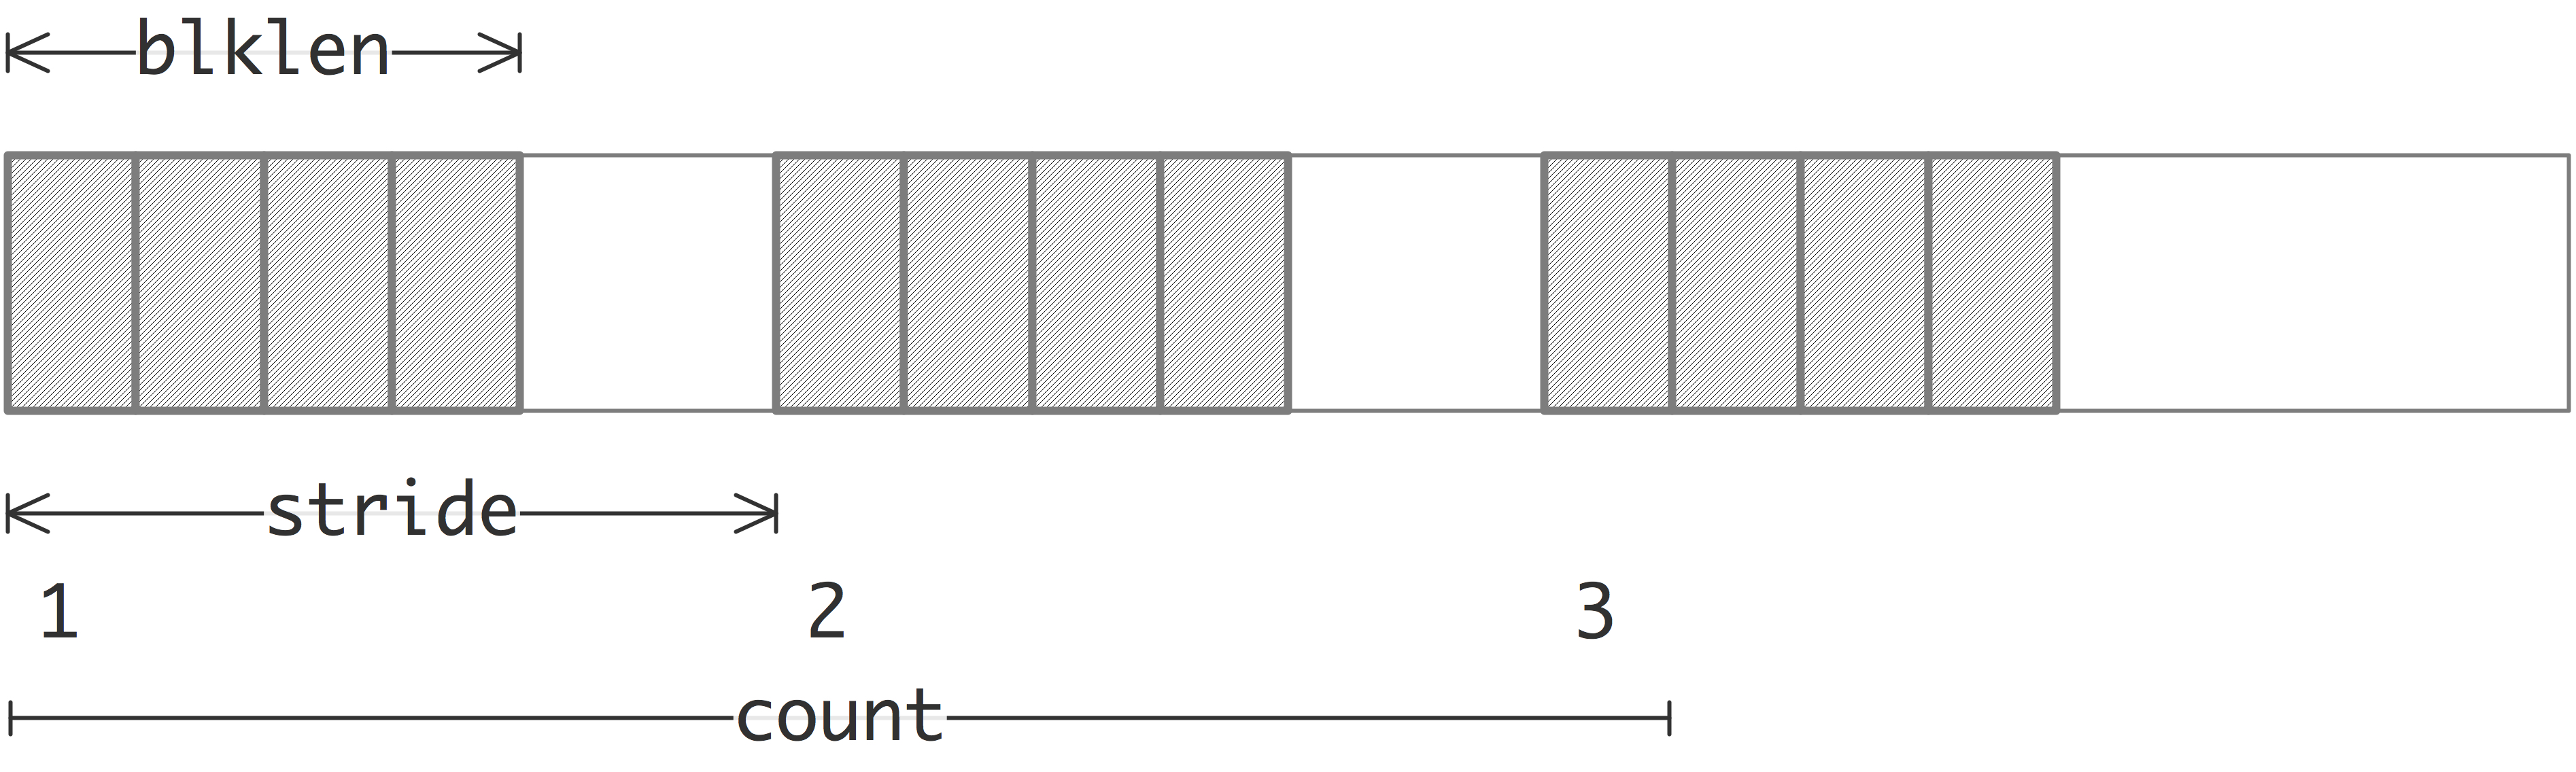
\includegraphics[scale=.12]{data-vector}
  \caption{A vector datatype is built up out of strided blocks of elements of a constituent type}
  \label{fig:data-vector}
\end{figure}
This is illustrated in figure~\ref{fig:data-vector}.

As an example of this datatype, consider the example of transposing
a matrix, for instance to convert between
C and Fortran arrays (see section~\HPSCref{sec:CFarrays}). Suppose that 
a processor has a matrix stored in~C, row-major, layout, and it needs
to send a column to another processor. If the matrix is declared as
\begin{verbatim}
  int M,N; double mat[M][N]
\end{verbatim}
then a column has $M$ blocks of one element, spaced $N$~locations apart.
In other words:
\begin{verbatim}
MPI_Datatype MPI_column;
MPI_Type_vector( 
    /* count= */ M, /* blocklength= */ 1, /* stride= */ N,
    MPI_DOUBLE, &MPI_column );
\end{verbatim}
Sending the first column is easy:
\begin{verbatim}
MPI_Send( mat, 1,MPI_column, ... );
\end{verbatim}
The second column is just a little trickier: you now need to pick out 
elements with the same stride, but starting at \n{A[0][1]}.
\begin{verbatim}
MPI_Send( &(mat[0][1]), 1,MPI_column, ... );
\end{verbatim}
You can make this marginally more efficient (and harder to read)
by replacing the index expression by \n{mat+1}.

\begin{exercise}
  Suppose you have a matrix of size $4N\times 4N$, and you want to
  send the elements \n{A[4*i][4*j]} with $i,j=0,\ldots,N-1$. How would
  you send these elements with a single transfer?
\end{exercise}

\begin{exercise}
  \label{ex:col-to-row}
  Allocate a matrix on processor zero, using Fortran column-major storage.
  Using $P$ sendrecv calls, distribute the rows of this matrix among the
  processors.
\end{exercise}

\Level 1 {Subarray type}

The vector datatype can be used for blocks in an array of dimension
more than~2 by using it recursively. However, this gets
tedious. Instead, there is an explicit subarray type
%
\mpiRoutineRef{MPI_Type_create_subarray}
%
This describes the dimensionality and extent of the array, and
the starting point (the `upper left corner') and extent of the subarray.

\Level 1 {Indexed type}
\commandref{data:indexed}

The indexed datatype, constructed with \indexmpishow{MPI_Type_indexed}
can send arbitrarily located elements from an array of a single datatype.
You need to supply an array of index locations, plus an array of blocklengths
with a separate blocklength for each index. The total number of elements sent
is the sum of the blocklengths.

\Level 1 {Struct type}
\commandref{data:struct}

The structure type, created with \indexmpishow{MPI_Type_create_struct},
can contain multiple data types.
\begin{figure}[ht]
  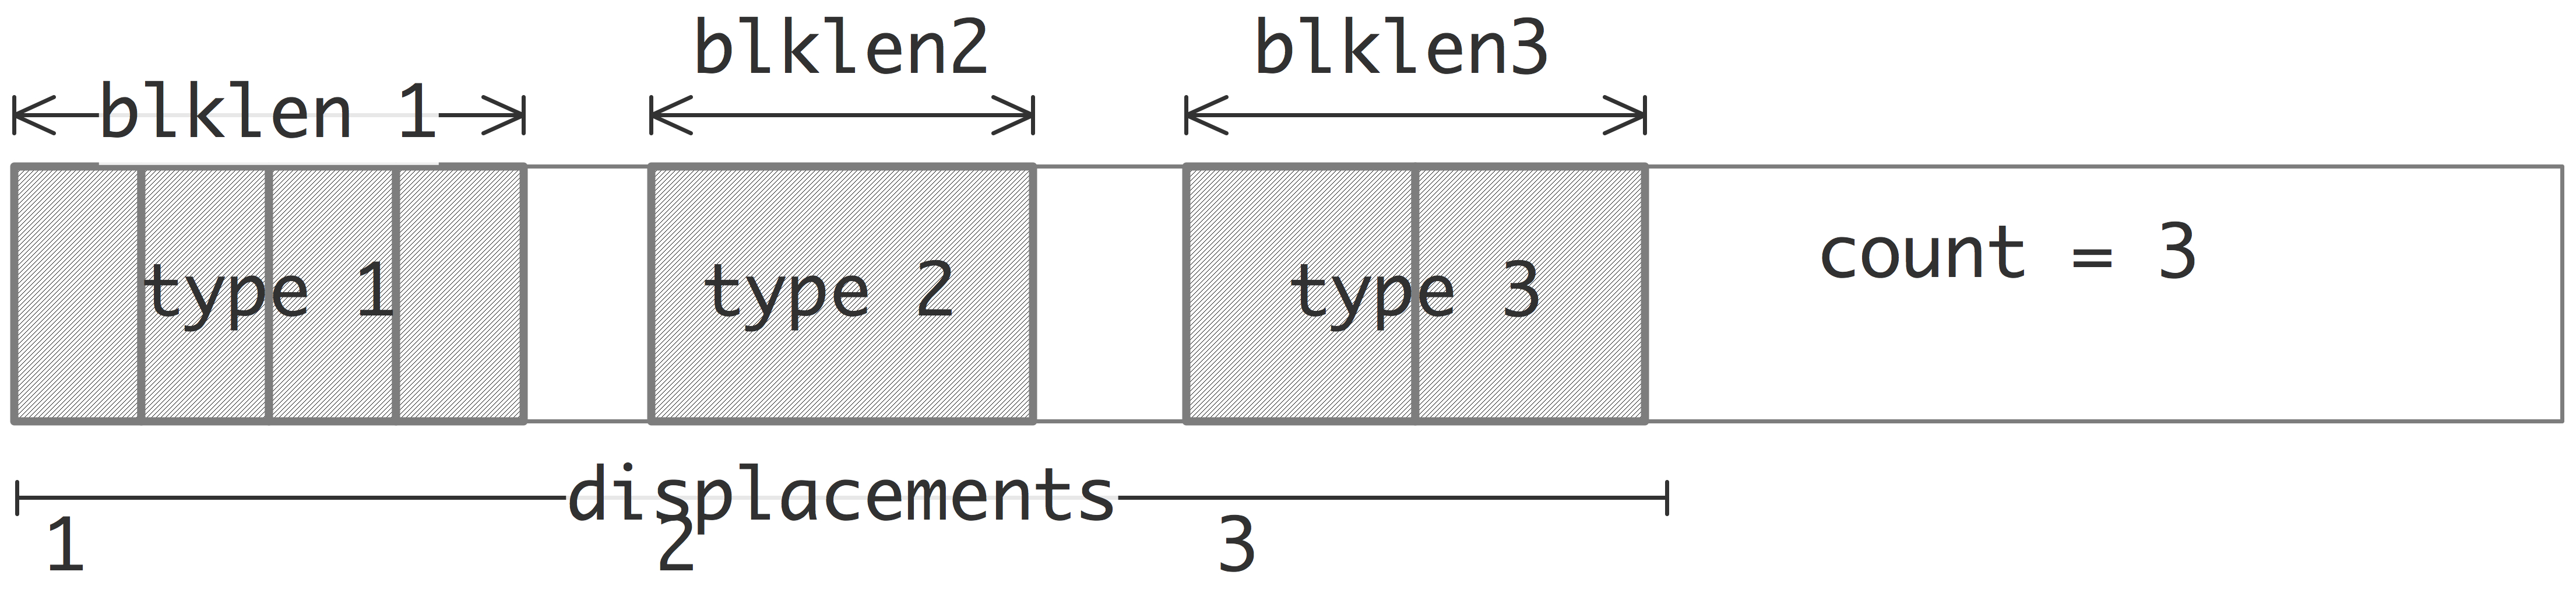
\includegraphics[scale=.11]{data-struct}
  \caption{The elements of an MPI Struct datatype}
  \label{fig:data-struct}
\end{figure}
The specification contains a `count' parameter that specifies how many blocks
there are in a single structure. For instance,
\begin{verbatim}
struct {
 int i;
 float x,y;
} point;
\end{verbatim}
has two blocks, one of a single integer, and one of two floats.
This is illustrated in figure~\ref{fig:data-struct}.

The structure type is very similar in functionality to \indexmpishow{MPI_Type_hindexed},
which uses byte-based indexing. The structure-based type is probably cleaner
in use.

\index{datatype!derived|)}

\Level 0 {Big data types}

The \n{size} parameter in MPI send and receive calls is of type integer,
meaning that it's maximally~$2^{31}-1$. These day computers are big enough
that this is a limitation. Derived types offer some way out: to send $10^{40}$
elements you would
\begin{itemize}
\item create a contiguous type with $10^{20}$ elements, and
\item send $10^{20}$ elements of that type.
\end{itemize}
This often works, but it's not perfect. For instance, the routine
\indexmpi{MPI_Get_elements} returns the total number of basic elements sent
(as opposed to \indexmpishow{MPI_Get_count} which would return the number
of elements of the derived type). Since its output argument is
of integer type, it can't store the right value.

The \indextermbus{MPI}{3} standard has addressed this
as follows.
\begin{itemize}
\item To preserve backwards compatibility, the \n{size} parameter keeps
  being of type integer.
\item The trick with sending elements of a derived type still works, but
\item There are new routines that can return the correct information about the
  total amount of data; for instance, \indexmpishow{MPI_Get_elements_x}
  returns its result as a \n{MPI_Count}.
\end{itemize}

\Level 0 {Packing}
\commandref{pack}

One of the reasons for derived datatypes is dealing with non-contiguous data.
In older communication libraries this could only be done by \indexterm{packing} data
from its original containers into a buffer, and likewise unpacking it at the
receiver into its destination data structures.

MPI offers this packing facility, partly for compatibility with such libraries,
but also for reasons of flexibility. Unlike with derived datatypes,
which transfers data atomically, packing routines add data sequentially
to the buffer and unpacking takes them sequentially. 

This means that 
one could pack an integer describing how many floating point numbers
are in the rest of the packed message. 
Correspondingly, the unpack routine could then investigate the first integer
and based on it unpack the right number of floating point numbers.

MPI offers the following:
\begin{itemize}
\item The \indexmpishow{MPI_Pack} command adds data to a send buffer;
\item the \indexmpishow{MPI_Unpack} command retrieves data from a receive buffer;
\item the buffer is sent with a datatype of \indexmpishow{MPI_PACKED}.
\end{itemize}

\index{datatype|)}

